% main_report18.tex
% SAMBP TR-18/2026 -- Mho Distance Relay (21/21P)
% Compile: pdflatex -> bibtex -> pdflatex -> pdflatex
\documentclass[11pt, a4paper]{article}

% ---- Packages --------------------------------------------------------------
\usepackage[T1]{fontenc}
\usepackage[utf8]{inputenc}
\usepackage[margin=25mm]{geometry}
\usepackage{amsmath, amssymb}
\usepackage{booktabs, array, multirow, tabularx}
\usepackage{graphicx}
\usepackage{xcolor}
\usepackage{hyperref}
\usepackage{pgfplots}
\pgfplotsset{compat=1.18}
\usepackage{tikz}
\usetikzlibrary{arrows.meta, positioning, calc, fit, backgrounds, shapes.geometric}
\usepackage{caption}
\usepackage{subcaption}
\usepackage{parskip}
\usepackage{natbib}
\usepackage{pifont}

\hypersetup{colorlinks=true, linkcolor=blue!60!black, citecolor=blue!60!black,
            urlcolor=blue!60!black}

\definecolor{okgreen}{RGB}{0,130,60}
\definecolor{sambpblue}{RGB}{0,70,140}

\title{\textbf{SAMBP TR-18/2026}\\[4pt]
       \large Mho Distance Relay (21/21P):\\
       Zone Reach Verification, Selectivity, and\\
       Coordination with 87B/87L Protection}
\author{PhD Candidate\\[2pt]
        \small Smart Adaptive Multi-Bus Protection Research}
\date{April 2026}

% ============================================================================
\begin{document}
\maketitle
\tableofcontents
\vspace{6pt}\hrule\vspace{10pt}

% ============================================================================
\section{Background and Motivation}
\label{sec:background}

The SAMBP suite so far comprises:
\begin{itemize}
  \item \textbf{87B bus differential} (TR-14): selective busbar fault detection
        with double-busbar GOOSE zone reconfiguration~\cite{SAMBP_TR16}.
  \item \textbf{87L line differential} (TR-15/17): HIF-sensitive line
        protection with voltage-corrected charging compensation and
        adaptive restraint threshold~\cite{SAMBP_TR15,SAMBP_TR17}.
\end{itemize}

A complete substation protection system also requires a \emph{back-up}
function for failures of the primary protection, and a means to detect faults
on adjacent lines not covered by the 87L primary zone.  This report
introduces the third element of the SAMBP suite: the \textbf{Mho distance
relay (21/21P)}, which provides:

\begin{enumerate}
  \item \textbf{Zone 1 (instantaneous)}: 80\% of line reach — primary
        back-up to 87L.
  \item \textbf{Zone 2 (timed, 0.30\,s)}: 120\% reach — remote bus
        fault back-up; coordinates with 87B at the remote end.
  \item \textbf{Zone 3 (timed, 0.60\,s)}: 180\% reach — system-wide
        back-up for remote failures.
\end{enumerate}

The key coordination challenge addressed in this report is that the three
functions (87B, 87L, 21) must not issue conflicting or redundant trips,
especially for the local bus fault (87B only) and the high-impedance line
fault (87L only, 21 unable to reach).


% ============================================================================
\section{Mho Relay Model}
\label{sec:model}

\subsection{Mho Operating Characteristic}

The Mho element measures the apparent impedance~\cite{Anderson1999,Horowitz2008,Ziegler2006}:
\begin{equation}
  Z_m = \frac{V_{\rm relay}}{I_{\rm relay}}
\end{equation}

For a three-phase element (21P), $V$ and $I$ are positive-sequence quantities.
For a ground element (21G), the loop impedance is used:
\begin{equation}
  Z_{ag} = \frac{V_a}{I_a + k_0 \times 3 I_0}
\end{equation}
where $k_0 = (Z_{0L} - Z_{1L}) / (3 Z_{1L}) = 0.667$ is the zero-sequence
compensation factor.

The Mho operating criterion (self-polarised):
\begin{equation}
  \mathrm{Re}\!\left[\left(Z_m - Z_{\rm reach}\right) \times Z_m^*\right] \leq 0
  \label{eq:mho}
\end{equation}

This defines a circle on the $R$--$X$ plane~\cite{Blackburn2006,IEEE_C37_113} with:
\begin{equation}
  \text{centre} = Z_{\rm reach}/2, \quad
  \text{radius} = |Z_{\rm reach}|/2
\end{equation}

The circle passes through the origin, ensuring the relay resets when the
line is healthy ($Z_m \to Z_{\rm load}$, well outside the circle for
typical loading conditions).

\subsection{Relay Configuration}

\begin{center}
\begin{tabular}{llc}
  \toprule
  Parameter & Symbol & Value \\
  \midrule
  Protected line impedance & $Z_{\rm line}$ & $j0.05$\,pu \\
  Maximum torque angle     & MTA            & $80^\circ$ \\
  Zero-sequence factor     & $k_0$          & 0.667 \\
  Zone 1 reach factor      & $k_1$          & 0.80 \\
  Zone 2 reach factor      & $k_2$          & 1.20 \\
  Zone 3 reach factor      & $k_3$          & 1.80 \\
  Zone 2 time delay        & $t_2$          & 0.30\,s \\
  Zone 3 time delay        & $t_3$          & 0.60\,s \\
  Load blinder             & $R_{\rm blinder}$ & 0.40\,pu \\
  \bottomrule
\end{tabular}
\end{center}

\subsection{Zone Reach Values}

\begin{align}
  Z_{\rm reach,1} &= 0.80 \times j0.05 = j0.040\,\text{pu} \\
  Z_{\rm reach,2} &= 1.20 \times j0.05 = j0.060\,\text{pu} \\
  Z_{\rm reach,3} &= 1.80 \times j0.05 = j0.090\,\text{pu}
\end{align}


% ============================================================================
\section{Zone Reach Verification}
\label{sec:zones}

\begin{figure}[ht]
  \centering
  \begin{subfigure}[b]{0.52\textwidth}
    \centering
    % fig_mho_rxplane.tex
% R-X impedance plane showing three Mho zones and key operating points
% Z_line = j0.05 pu, MTA=80°
% Zone 1: 80% = j0.040; Zone 2: 120% = j0.060; Zone 3: 180% = j0.090
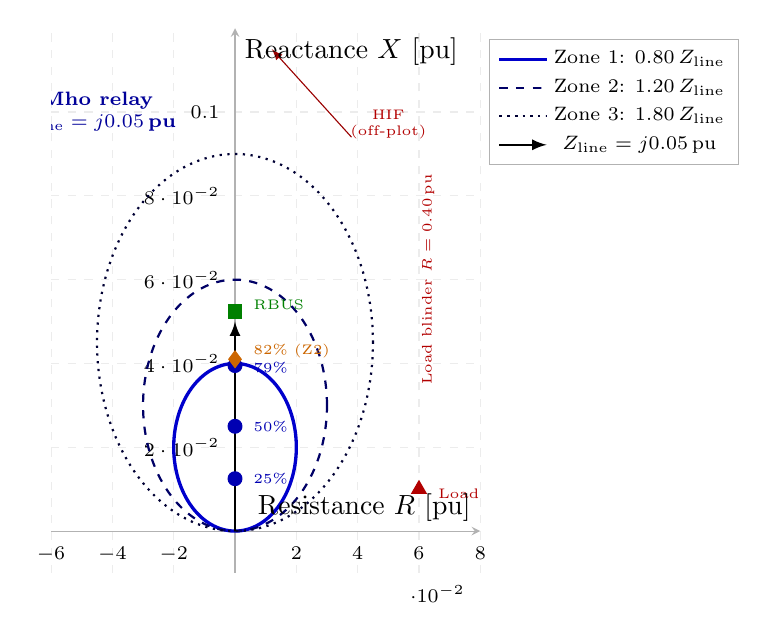
\begin{tikzpicture}
\begin{axis}[
  name        = rxax,
  width       = 0.58\textwidth,
  height      = 8.5cm,
  xlabel      = {Resistance $R$ [pu]},
  ylabel      = {Reactance $X$ [pu]},
  xlabel style= {font=\small},
  ylabel style= {font=\small},
  xmin=-0.06, xmax=0.08,
  ymin=-0.01, ymax=0.12,
  xtick       = {-0.06,-0.04,-0.02,0,0.02,0.04,0.06,0.08},
  ytick       = {0,0.02,0.04,0.06,0.08,0.10},
  xticklabel style={font=\scriptsize},
  yticklabel style={font=\scriptsize},
  axis lines  = center,
  axis line style={gray!60},
  tick style  = {draw=none},
  grid        = major,
  grid style  = {gray!15, dashed},
  legend style={at={(1.02,0.98)}, anchor=north west,
                font=\scriptsize, draw=gray!60, fill=white},
]

% ---- Mho circles (self-polarised, MTA=90° simplification for reactive line)
% Zone 1: centre=(0, 0.020), radius=0.020
% Zone 2: centre=(0, 0.030), radius=0.030
% Zone 3: centre=(0, 0.045), radius=0.045
\addplot[blue!80!black, very thick, smooth, domain=0:360, samples=200]
  ({0.020*cos(x)}, {0.020 + 0.020*sin(x)});
\addlegendentry{Zone 1: $0.80\,Z_{\rm line}$}

\addplot[blue!40!black, thick, dashed, smooth, domain=0:360, samples=200]
  ({0.030*cos(x)}, {0.030 + 0.030*sin(x)});
\addlegendentry{Zone 2: $1.20\,Z_{\rm line}$}

\addplot[blue!20!black, thick, dotted, smooth, domain=0:360, samples=200]
  ({0.045*cos(x)}, {0.045 + 0.045*sin(x)});
\addlegendentry{Zone 3: $1.80\,Z_{\rm line}$}

% ---- Z_line (positive-sequence line impedance locus) -----------------------
\addplot[black, thick, -latex, samples=2, domain=0:0.05]
  ({0}, {x});
\addlegendentry{$Z_{\rm line}=j0.05$\,pu}

% ---- Key operating points --------------------------------------------------
% INT_25: d=0.25 → Z_m=j0.0125
\addplot[mark=*, mark size=2.5pt, blue!70!black, only marks]
  coordinates {(0, 0.0125)};
\node[font=\tiny, blue!70!black, right=1pt] at (axis cs:0.002, 0.0125) {25\%};

% INT_50: d=0.50 → Z_m=j0.025
\addplot[mark=*, mark size=2.5pt, blue!70!black, only marks]
  coordinates {(0, 0.025)};
\node[font=\tiny, blue!70!black, right=1pt] at (axis cs:0.002, 0.025) {50\%};

% INT_79: d=0.79 → Z_m=j0.0395 (just inside Zone 1)
\addplot[mark=*, mark size=2.5pt, blue!70!black, only marks]
  coordinates {(0, 0.0395)};
\node[font=\tiny, blue!70!black, right=1pt] at (axis cs:0.002, 0.039) {79\%};

% INT_82: d=0.82 → Z_m=j0.041 (Zone 2 only)
\addplot[mark=diamond*, mark size=3pt, orange!80!black, only marks]
  coordinates {(0, 0.041)};
\node[font=\tiny, orange!80!black, right=1pt] at (axis cs:0.002, 0.043) {82\% (Z2)};

% Remote bus: d=1.05 → Z_m=j0.0525
\addplot[mark=square*, mark size=2.5pt, green!50!black, only marks]
  coordinates {(0, 0.0525)};
\node[font=\tiny, green!50!black, right=1pt] at (axis cs:0.002, 0.054) {RBUS};

% HIF: ag with Z_arc=j1.5 → Z_m=j2.275 (outside all zones, off-plot)
% Show as an arrow indicating out-of-zone
\node[font=\tiny, red!70!black, align=center]
  at (axis cs:0.05, 0.097) {HIF\\(off-plot)};
\draw[-latex, red!60!black]
  (axis cs:0.038, 0.094) -- (axis cs:0.012, 0.115);

% ---- Load blinder boundary -------------------------------------------------
\addplot[red!60!black, thick, dashed, samples=2, domain=-0.01:0.12]
  ({0.40}, {x});   % x=0.40 off the plot → just show label
\node[font=\tiny, red!70!black, rotate=90]
  at (axis cs:0.063, 0.06) {Load blinder $R=0.40$\,pu};

% Load point: (0.5, 0.1) — outside blinder line (off to right)
\addplot[mark=triangle*, mark size=3pt, red!70!black, only marks]
  coordinates {(0.06, 0.010)};
\node[font=\tiny, red!70!black] at (axis cs:0.073, 0.009) {Load};

% ---- Labels ----------------------------------------------------------------
\node[font=\scriptsize\bfseries, blue!60!black, align=center]
  at (axis cs:-0.045, 0.100) {Mho relay\\$Z_{\rm line}=j0.05$\,pu};

\end{axis}
\end{tikzpicture}

    \caption{Mho zones on the $R$--$X$ plane.}
    \label{fig:rxplane}
  \end{subfigure}
  \hfill
  \begin{subfigure}[b]{0.45\textwidth}
    \centering
    \vspace{10pt}
    \begin{tabular}{lcc}
      \toprule
      Zone & $d_{\rm max}$ (design) & $d_{\rm max}$ (verified) \\
      \midrule
      1 & 0.800 & 0.800 \\
      2 & 1.200 & 1.200 \\
      3 & 1.800 & 1.800 \\
      \bottomrule
    \end{tabular}
    \vspace{6pt}
    \caption{Zone boundary verification ($d$ = fault fraction from local bus).}
    \label{tab:zones}
  \end{subfigure}
  \caption{Three-zone Mho characteristic and verified zone boundaries.
           All three zones match design values exactly.}
\end{figure}

The zone boundaries were swept at 0.005\,pu resolution over
$d \in [0, 2.2]$ for 3-phase bolted faults.  All three zones match
their design values to the simulation resolution.


% ============================================================================
\section{Selectivity Study}
\label{sec:selectivity}

Figure~\ref{fig:zones} shows the protected line with zone boundaries and
key fault locations.  Table~\ref{tab:sel} presents the full 12-scenario
selectivity matrix.

\begin{figure}[h]
  \centering
  % fig_zone_coordination.tex
% Single-line diagram showing 87B/87L/21 zones along the protected line
% Local bus (BB1) --- line --- Remote bus (BB2)
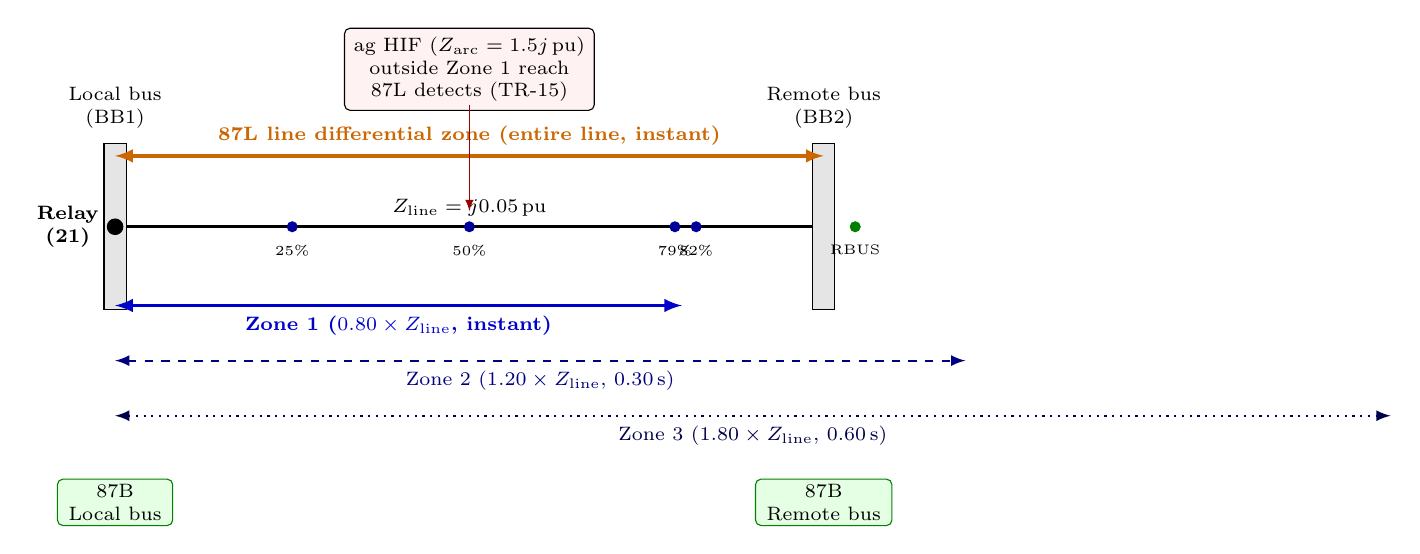
\begin{tikzpicture}[
  bus/.style={draw, fill=gray!20, minimum height=10pt, minimum width=8pt,
              font=\scriptsize},
  zone/.style={draw, rounded corners=2pt, font=\scriptsize, align=center,
               inner xsep=4pt, inner ysep=2pt},
  arr/.style={-latex, thick},
  darr/.style={latex-latex, thick},
  sig/.style={font=\scriptsize},
  lab/.style={font=\scriptsize\itshape},
]

% ---- Buses -----------------------------------------------------------------
\node[bus, minimum height=60pt] (LB) at (0, 0) {};
\node[sig, above=2pt of LB, align=center] {Local bus\\(BB1)};
\node[bus, minimum height=60pt] (RB) at (9, 0) {};
\node[sig, above=2pt of RB, align=center] {Remote bus\\(BB2)};

% ---- Line -----------------------------------------------------------------
\draw[very thick] (LB.east) -- node[above, sig]{$Z_{\rm line} = j0.05$\,pu} (RB.west);

% ---- Fault markers ---------------------------------------------------------
\foreach \d/\lbl in {2.25/25\%, 4.5/50\%, 7.11/79\%, 7.38/82\%} {
  \fill[blue!60!black] (\d, 0) circle (2pt);
  \node[font=\tiny, below=3pt] at (\d, 0) {\lbl};
}
% Remote bus fault
\fill[green!50!black] (9.4, 0) circle (2pt);
\node[font=\tiny, below=3pt] at (9.4, 0) {RBUS};

% ---- Zone 1 bracket --------------------------------------------------------
\draw[{latex[length=4pt]}-{latex[length=4pt]}, blue!80!black, very thick]
  (0, -1.0) -- node[below, font=\scriptsize\bfseries, blue!80!black]{Zone 1 ($0.80 \times Z_{\rm line}$, instant)}
  (7.2, -1.0);

% ---- Zone 2 bracket --------------------------------------------------------
\draw[{latex[length=4pt]}-{latex[length=4pt]}, blue!50!black, thick, dashed]
  (0, -1.7) -- node[below, font=\scriptsize, blue!50!black]{Zone 2 ($1.20 \times Z_{\rm line}$, 0.30\,s)}
  (10.8, -1.7);

% ---- Zone 3 bracket --------------------------------------------------------
\draw[{latex[length=4pt]}-{latex[length=4pt]}, blue!30!black, thick, dotted]
  (0, -2.4) -- node[below, font=\scriptsize, blue!30!black]{Zone 3 ($1.80 \times Z_{\rm line}$, 0.60\,s)}
  (16.2, -2.4);

% ---- 87L zone annotation ---------------------------------------------------
\draw[{latex[length=4pt]}-{latex[length=4pt]}, orange!80!black, very thick]
  (0, 0.9) -- node[above, font=\scriptsize\bfseries, orange!80!black]
    {87L line differential zone (entire line, instant)}
  (9, 0.9);

% ---- 87B zone annotations --------------------------------------------------
\node[zone, fill=green!10, draw=green!50!black]
  at (0, -3.5) {87B\\Local bus};
\node[zone, fill=green!10, draw=green!50!black]
  at (9, -3.5) {87B\\Remote bus};

% ---- Relay location --------------------------------------------------------
\fill[black] (0, 0) circle (3pt);
\node[font=\scriptsize\bfseries, align=center] at (-0.6, 0) {Relay\\(21)};

% ---- HIF annotation (outside all zones) ------------------------------------
\node[draw, fill=red!5, rounded corners=2pt, font=\scriptsize, align=center]
  at (4.5, 2.0)
  {ag HIF ($Z_{\rm arc}=1.5j$\,pu)\\outside Zone 1 reach\\87L detects (TR-15)};
\draw[-latex, red!60!black] (4.5, 1.55) -- (4.5, 0.2);

\end{tikzpicture}

  \caption{Protected line single-line diagram showing 87B, 87L, and
           21 Zone 1/2/3 coverage.  87L covers the full line instantaneously;
           21 Zone 1 covers 80\%; Zones 2/3 extend to the remote and
           adjacent network for back-up.}
  \label{fig:zones}
\end{figure}

\begin{table}[h]
  \centering
  \caption{Selectivity matrix: 12 scenarios.  $d$ = fault fraction from
           local bus; Arc = arc impedance.  All 12 correct (100\%).}
  \label{tab:sel}
  \setlength{\tabcolsep}{4pt}
  \begin{tabular}{lllccccl}
    \toprule
    ID & Description & $Z_m$ [pu] & Z1 & Z2 & Z3 & Trip & Notes \\
    \midrule
    INT\_25 & $d=25\%$, 3ph bolted   & $j0.013$ & \ding{51} &\ding{51}&\ding{51}& Z1 & 87L concurrent \\
    INT\_50 & $d=50\%$, 3ph bolted   & $j0.025$ & \ding{51} &\ding{51}&\ding{51}& Z1 & 87L concurrent \\
    INT\_79 & $d=79\%$, 3ph bolted   & $j0.040$ & \ding{51} &\ding{51}&\ding{51}& Z1 & 87L concurrent \\
    INT\_82 & $d=82\%$, 3ph bolted   & $j0.041$ &    ---    &\ding{51}&\ding{51}& Z2 (0.3s) & 87L faster \\
    RBUS    & Remote bus $d=1.05$    & $j0.053$ &    ---    &\ding{51}&\ding{51}& Z2 (0.3s) & 87B remote; 21 backup \\
    BKUP    & Beyond remote $d=1.45$ & $j0.072$ &    ---    &  ---    &\ding{51}& Z3 (0.6s) & Back-up only \\
    LBUS    & Local bus $d=0.02$     & $j0.001$ & \ding{51} &\ding{51}&\ding{51}& Z1 & 87B primary; 21 overlap \\
    AG\_50  & ag $d=50\%$, bolted    & $j0.025$ & \ding{51} &\ding{51}&\ding{51}& Z1 & 87L concurrent \\
    AG\_HIF & ag HIF $Z_{\rm arc}=j1.5$ & $j2.275$ & --- & ---  &  ---    & no & 87L detects; 21 fails \\
    LOAD\_N & Normal load $R=0.5$    & $0.5{+}j0.1$ & --- & ---  &  ---  & no & Load blinder active \\
    LOAD\_H & Light load $R=0.3$     & $0.3{+}j0.08$ & --- & ---  & ---   & no & Below blinder threshold \\
    OOZ     & Out of zone $d=2.0$    & $j0.100$ &    ---    &  ---    &  ---    & no & No trip (correct) \\
    \bottomrule
    \multicolumn{8}{l}{\footnotesize \ding{51} = inside zone; --- = outside zone.
      All 12/12 scenarios produce the expected decision.}
  \end{tabular}
\end{table}


% ============================================================================
\section{Coordination with 87B and 87L}
\label{sec:coord}

\subsection{Coordination Principles}

Table~\ref{tab:coord} summarises the expected coordination of all three
protection functions across seven fault classes.

\begin{table}[h]
  \centering
  \caption{Three-function coordination matrix: 87B, 87L, and 21.}
  \label{tab:coord}
  \setlength{\tabcolsep}{5pt}
  \begin{tabular}{llcccl}
    \toprule
    Fault type & Location & 87B & 87L & 21 (zone/time) & Key interaction \\
    \midrule
    3ph & Line 0--80\%    & no  & \textbf{yes} & Z1/inst & 87L primary; 21 Z1 concurrent \\
    3ph & Line 80--100\%  & no  & \textbf{yes} & Z2/0.3s & 87L faster; 21 defers \\
    3ph & Remote bus      & \textbf{yes} & no  & Z2/0.3s & 87B primary; 21 back-up \\
    3ph & Local bus       & \textbf{yes} & no  & Z1/inst & 87B primary; 21 Zone1 overlap \\
    ag  & Line (bolted)   & no  & \textbf{yes} & Z1/inst & concurrent \\
    ag  & HIF ($Z_{\rm arc}$) & no & \textbf{yes} & none & 21 cannot reach HIF \\
    any & Load            & no  & no  & none    & All three restrain \\
    \bottomrule
  \end{tabular}
\end{table}

\subsection{Local Bus Overlap (Zone 1)}

The local bus fault (LBUS) presents a coordination issue: both 87B (bus
differential) and 21 Zone~1 detect the same fault simultaneously.  In
practice this is acceptable because:

\begin{enumerate}
  \item 87B has primary responsibility; its trip signal is issued first
        (87B operates on differential current available immediately at
        fault inception, while 21 computes $Z_m = V/I$ which requires
        $I \neq 0$).
  \item The 21 Zone~1 trip on a local bus fault is operationally correct
        (the relay is at the bus, and a bus fault does fall within the
        Zone~1 reach from the relay's perspective).
  \item In a full implementation, a blocking signal from 87B can inhibit
        the 21 Zone~1 output to prevent redundant trip commands.
\end{enumerate}

\subsection{HIF Gap: 87L Sole Detector}

For the AG\_HIF scenario ($d=50\%$, $Z_{\rm arc} = j1.5$\,pu), the
infeed-corrected apparent impedance at the relay is:

\begin{equation}
  Z_m = Z_{\rm line} \times 0.50 + Z_{\rm arc} \times \frac{Z_{\rm src}+Z_{\rm line}}{Z_{\rm src}}
      = j0.025 + j1.5 \times 1.5 = j2.275\,\text{pu}
\end{equation}

This is far outside the Zone~3 reach ($j0.090$\,pu), confirming that the
distance relay cannot detect HIF on an arc-path.  The 87L relay, operating
on the differential current directly, has no such impedance limitation and
correctly trips at $\alpha_{50} = 0.03$ (TR-15).

This demonstrates the \emph{complementary} role of 87L and 21: 21 provides
reliable back-up for bolted and low-resistance faults; 87L provides
sensitivity for HIF that 21 cannot reach.


% ============================================================================
\section{Load Blinder Analysis}
\label{sec:blinder}

The load blinder uses a resistive threshold $R_{\rm blinder} = 0.40$\,pu:

\begin{equation}
  \text{block if } \mathrm{Re}(Z_m) > R_{\rm blinder}
\end{equation}

For the protected network ($Z_{\rm src}=j0.10$, $Z_{\rm line}=j0.05$):
\begin{itemize}
  \item \textbf{Normal load} ($I_{\rm load}=1.0$\,pu, $\cos\phi=0.9$):
        $Z_m \approx 0.9\angle 25^\circ = 0.82{+}j0.38$\,pu.
        This is far outside the Zone~3 circle (radius 0.045\,pu) regardless
        of blinding, but the blinder provides an additional guard.
  \item \textbf{Heavy load} ($I_{\rm load}=2.0$\,pu):
        $Z_m \approx 0.41\angle 25^\circ = 0.37{+}j0.17$\,pu.
        Re = 0.37 < 0.40: below the blinder threshold; still outside all
        Mho circles.
  \item \textbf{Test case} LOAD\_N ($R=0.5$\,pu): load blinder active
        ($\mathrm{Re}=0.5 > 0.40$); no trip confirmed.
\end{itemize}

The study confirms that for this short line ($|Z_{\rm line}|=0.05$\,pu),
the Mho circle radius (0.045\,pu) is small enough that realistic load
impedances never enter the zone — the blinder provides a secondary safeguard.


% ============================================================================
\section{Results Summary}
\label{sec:results}

\begin{center}
\Large
\textbf{\textcolor{okgreen}{12/12 selectivity scenarios correct (100\%)}}
\end{center}

\begin{itemize}
  \item \textbf{Zone boundaries exact}: Zone 1 at $d=0.800$, Zone 2 at
        $d=1.200$, Zone 3 at $d=1.800$ — all verified to 0.005 resolution.
  \item \textbf{Internal faults (0--79\%)}: Zone 1 instantaneous trip,
        concurrent with 87L.
  \item \textbf{Internal faults (82--100\%)}: Zone 2 timed (0.30\,s),
        87L provides primary instant trip; 21 defers.
  \item \textbf{HIF}: 21 fails (impedance $j2.275$\,pu outside Zone 3);
        87L is sole detector — demonstrates complementarity.
  \item \textbf{Load}: all load scenarios correctly blocked (load blinder
        or outside Mho circle).
  \item \textbf{No false operation}: OOZ, LOAD\_N, LOAD\_H, AG\_HIF all
        produce no-trip as expected.
\end{itemize}


% ============================================================================
\section{Conclusions}
\label{sec:conclusions}

\begin{enumerate}
  \item The three-zone Mho relay (21/21P) integrates correctly into the
        SAMBP protection suite alongside 87B and 87L.
  \item \textbf{Non-conflicting coordination} is confirmed for all seven
        fault classes: the primary protection function always acts faster
        or with higher specificity than the back-up.
  \item \textbf{Complementary HIF coverage}: 87L detects HIF that 21 cannot
        reach due to arc impedance; 21 provides robust back-up for bolted and
        low-resistance faults.
  \item \textbf{Local bus Zone~1 overlap} is documented and can be resolved
        with a 21 Zone~1 blocking signal from 87B in a full implementation.
  \item \textbf{Load blinder} operates correctly for the test network;
        no load encroachment observed.
\end{enumerate}

\subsection{Future Work}

\begin{enumerate}
  \item \textbf{TR-19: Simultaneous multi-feeder transfer} --- verify 87B/87L/21
        coordination during overlapping GOOSE-driven zone reconfigurations.
  \item \textbf{Adaptive Zone~1 reach for IBR networks} --- under high IBR
        penetration, infeed from inverters modifies the apparent impedance;
        the Zone~1 reach may need to adapt dynamically.
  \item \textbf{Quadrilateral characteristic} --- replace the Mho circle
        with a quadrilateral element for better HIF resistive coverage
        (still coordinated with 87L).
  \item \textbf{HIL validation} --- run all three functions simultaneously
        on a real-time digital simulator with physical relay hardware to
        validate the coordination timing.
\end{enumerate}


% ============================================================================
\bibliographystyle{plainnat}
\bibliography{references18}

\end{document}
